%%%%%%%%%%%%%%%%%%%%%%%%%%%%%%%%%%%%%%%%%%%%%%
% Header
\documentclass[11pt]{report}
\usepackage[english]{babel}
\usepackage[utf8x]{inputenc}
\PassOptionsToPackage{hyphens}{url}\usepackage{hyperref}
\usepackage{graphicx}
\usepackage{fullpage}
\usepackage{nicefrac}
\usepackage[lastexercise]{exercise}
\usepackage[dvipsnames]{xcolor}
\usepackage{listings}
\usepackage{enumitem}
\graphicspath{ {./img/} }

\setlength{\parindent}{0cm}

\renewcommand{\ExerciseHeader}{\large\textbf{\ExerciseName~\ExerciseHeaderNB} - \textbf{\ExerciseTitle}\medskip}

\renewcommand{\ExePartHeader}{\medskip\textbf{\ExePartName\ExePartHeaderNB\ExePartHeaderTitle\medskip}}

\begin{document}
%%%%%%%%%%%%%%%%%%%%%%%%%%%%%%%%%%%%%%%%%%%%%%
\title{Exercises -- Week 9: New Title}
\subsubsection*{EMAT10007 -- Introduction to Computer Programming}
\section*{\Large Exercises -- Week 9. Matplotlib}

\subsection*{\Large 9.1 Plotting}
\subsection*{Essential Questions}

\textbf{Note:} A widely-used way to import the matplotlib module is by adding the following line at the start of your code: {\tt import matplotlib.pyplot as plt}. Any function belonging to the  matplotlib module can then be accessed by writing, for example, {\tt plt.plot()}.


\begin{Exercise}[title= Line and scatter graphs] \label{Ex:Variables}
  
	\Question{Create two lists of integers named {\tt x} and {\tt y} with the following values: \\
	{\tt x = [0,2,4,5,8,10,13]}\\
	{\tt y = [1,3,3,3,4,5,6]}\\
	Plot a line graph of {\tt y} against  {\tt x} .}\\
	\textbf {Hint:}	Remember to use {\tt plt.show()} to display the graph.
	\Question{Modify your code so the resulting graph looks like the graph below:}
	
    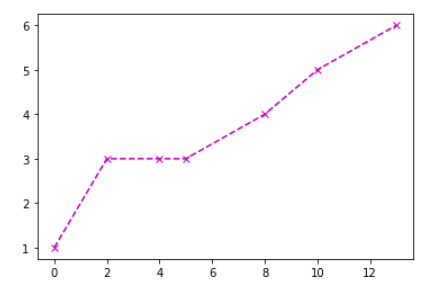
\includegraphics[height=5.5cm]{lineGraph}
    \label{fig:lineGraph}

	\Question{On the same axes, plot the graph of {\tt f} against  {\tt x} so it looks like the graph below:\\
	{\tt f = [-3,0,1,0,4,6,7]}}\\
	
	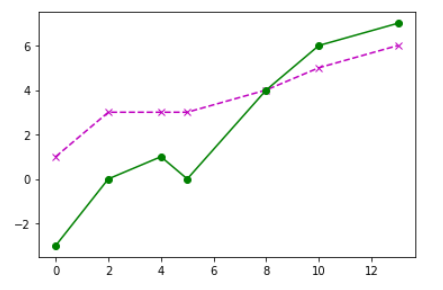
\includegraphics[height=5.5cm]{linesGraph}
    \label{fig:linesGraph}
    
	\Question{Now alter your graph so it has the following} 
	\begin{itemize}
	    \item title: {\tt Plot of y,f vs x}
	    \item x axis label: {\tt x}
	    \item legend indicating which line is {\tt y} data and which is {\tt f}
	    
	  \end{itemize}
	  
	  \Question{Save your plot as a .pdf file}

\end{Exercise}

%\newpage


\begin{Exercise}[title= Histograms and importing data] \label{Ex:Variables}
	\Question{Create a function named {\tt diceRolls} that takes the number of 6-sided dice rolls, {\tt n} as an input argument and return the results of the dice rolls. \\
	\textbf{Hint:} Use the numpy {\tt np.random.randint()} function.}
	
	\Question{Modify the {\tt diceRolls} function so it saves the results in a file diceRolls.csv.\\
	\textbf{Hint:} Remember to import any modules you need at the start of your code.}

	\Question{Call the {\tt diceRolls} function, choosing a value for {\tt n}. Then import the dice rolls from your diceRolls.csv file and save it as a numpy array, {\tt data}. Print {\tt data}.}
	\Question{Visualise the data in the {\tt data} array. First, try using {\tt plt.plot()}. This shows the results of each dice roll, but is slightly confusing to look at. }
	\Question{Now, let's try to represent the distribution of dice rolls using a histogram. Use {\tt plt.hist()}  and {\tt plt.show()} to visualise the histogram. \\ {\bf Hint:} Try using the different optional arguments (e.g. {\tt align}) to change the appearance of the plot  (https://matplotlib.org/stable/api/\_as\_gen/matplotlib.pyplot.hist.html)}
	\Question{Add a title and x and y axis labels to your histogram. Try running your code with n = 10, 100, 1,000 and 10,000 to see if/how the distribution of dice rolls changes.}
	
	\Question{Save your plot as a .png file}

\end{Exercise}

\subsection*{Advanced Questions}

The file `douglas\_data.csv` contains a data set of recorded parameters for a sample of wooden beams. Open the file using a spreadsheet program or text editor and look at the data. Which rows and columns contain non-numeric data?

\begin{enumerate}[label=(\Alph*)]
    
    \item   \\
    Import the data from `douglas\_data.csv`:
    \begin{itemize}
        \item using {\tt np.loadtxt}
        \item using using the default data type ({\tt float})
        \item specifying the correct delimiter
        \item excluding the rows and columns containing non-numeric data.
    \end{itemize}
    {\bf Note:} The use of scientific notation can be suppressed by:
    \begin{verbatim}
        np.set_printoptions(suppress=True)
    \end{verbatim}
    
    \item Select the first 10 rows of the array to create a new array.\\
    The data in the last column is in units $\mathrm{N/mm}^2$.\\
    Convert the data in this column to units $\mathrm{N/m}^2$.\\

    \item The area of each beam in the data set is 0.01 $\mathrm{m^2}$.\\
    The density of each beam (kg/m$^3$) is given in the fifth column. \\
    The height of each beam (cm) is given in the sixth column. \\
    Add a new column to the array that contains mass of each beam (kg) using:

    mass $=$ area $\times$ height $\times$ density
    
    \item Create two sub-plots:
    \begin{itemize}
        \item a scatter graph of  bend strength against knot ratio 
        \item a bar chart showing the mass of each sample
    \end{itemize}

\end{enumerate}

\subsection*{\Large 9.2 Curve Fitting}

\subsection*{Essential Questions}

\begin{Exercise}[title= Polynomials] \label{Ex:Variables}
	\Question{Generate two numpy arrays of 20 random floating point number ranging from 1 to 10, named {\tt x} and {\tt y}. Sort the lists so they are both in ascending order.\\
	\textbf{Hint:} Use {\tt np.random.uniform()} and {\tt np.sort()}.}
	\Question{Display the data from the sorted {\tt x} and {\tt y} functions as a scatter plot.}
	\Question{Use {\tt polyfit} to determine the coefficients of a second degree polynomial ({\tt deg = 2}) fit to your {\tt x} and {\tt y} data. Then use {\tt poly1d} to generate a new array of fitted data, {\tt yfit}.}
	\Question{Show the fitted data as a line graph on the same axes as the raw data.}
	\Question{Modify your code so the polynomial fit is now of the 5th degree.}
	\Question{How does this affect the fit to your data? \\Compare the root mean square error (RMSE) of the fitted data for the 2nd and 5th degree polynomial.}
\end{Exercise}

\subsection*{Advanced Questions}

The file `data/douglas\_data.csv` contains a data set of recorded parameters for a sample of wooden beams.

\begin{enumerate}[label=(\Alph*)]
    \item Import the data from `douglas\_data.csv`:
    \begin{itemize}
        \item using {\tt np.loadtxt}
        \item using using the default data type ({\tt float})
        \item specifying the correct delimiter
        \item excluding the rows and columns containing non-numeric data.
    \end{itemize}
    {\bf Note:} The use of scientific notation can be suppressed by:
    \begin{verbatim}
        np.set_printoptions(suppress=True)
    \end{verbatim}
    
    \item Plot a scatter graph of bend strength against knot ratio. 
    \item Can you think of a mathematical function that looks like it could fit this data? Define the mathematical function as a Python function and use {\tt curve\_fit} to fit a function to the data.\\  {\bf Hint:} Remember to import {\tt curve\_fit} from {\tt scipy.optimize}.  
    \item Use the Python function you defined to generate some fitted data. 
    \item Plot the fitted data as a line plot on the same axes as the raw data. Label the axes.
    \item Show the equation of the fitted line in the figure legend.
    \item What is the root mean square error (RMSE) of the fitted function? 
\end{enumerate}

\end{document}